%!TEX TS-program = xelatex
\documentclass[]{friggeri-cv}
\usepackage{afterpage}
\usepackage{hyperref}
\usepackage{color}
\usepackage{xcolor}
\usepackage{smartdiagram}
\usepackage{fontspec}
% if you want to add fontawesome package
% you need to compile the tex file with LuaLaTeX
% References:
%   http://texdoc.net/texmf-dist/doc/latex/fontawesome/fontawesome.pdf
%   https://www.ctan.org/tex-archive/fonts/fontawesome?lang=en
%\usepackage{fontawesome}
\usepackage{metalogo}
\usepackage{dtklogos}
\usepackage[utf8]{inputenc}
\usepackage{tikz}
\usetikzlibrary{mindmap,shadows}
\hypersetup{
    pdftitle={},
    pdfauthor={},
    pdfsubject={},
    pdfkeywords={},
    colorlinks=false,           % no lik border color
    allbordercolors=white       % white border color for all
}
\smartdiagramset{
    bubble center node font = \footnotesize,
    bubble node font = \footnotesize,
    % specifies the minimum size of the bubble center node
    bubble center node size = 0.5cm,
    %  specifies the minimum size of the bubbles
    bubble node size = 0.5cm,
    % specifies which is the distance among the bubble center node and the other bubbles
    distance center/other bubbles = 0.3cm,
    % sets the distance from the text to the border of the bubble center node
    distance text center bubble = 0.5cm,
    % set center bubble color
    bubble center node color = pblue,
    % define the list of colors usable in the diagram
    set color list = {lightgray, materialcyan, orange, green, materialorange, materialteal, materialamber, materialindigo, materialgreen, materiallime},
    % sets the opacity at which the bubbles are shown
    bubble fill opacity = 0.6,
    % sets the opacity at which the bubble text is shown
    bubble text opacity = 0.5,
}

\addbibresource{bibliography.bib}
\RequirePackage{xcolor}
\definecolor{pblue}{HTML}{0395DE}

\begin{document}

\header{-----------  Jaziel David}{  Flores Rodríguez.}
      {Matemático-Físico y Programador. }
      
% Fake text to add separator      
\fcolorbox{white}{gray}{\parbox{\dimexpr\textwidth-2\fboxsep-2\fboxrule}{%
.....
}}

% In the aside, each new line forces a line break
\begin{aside}
  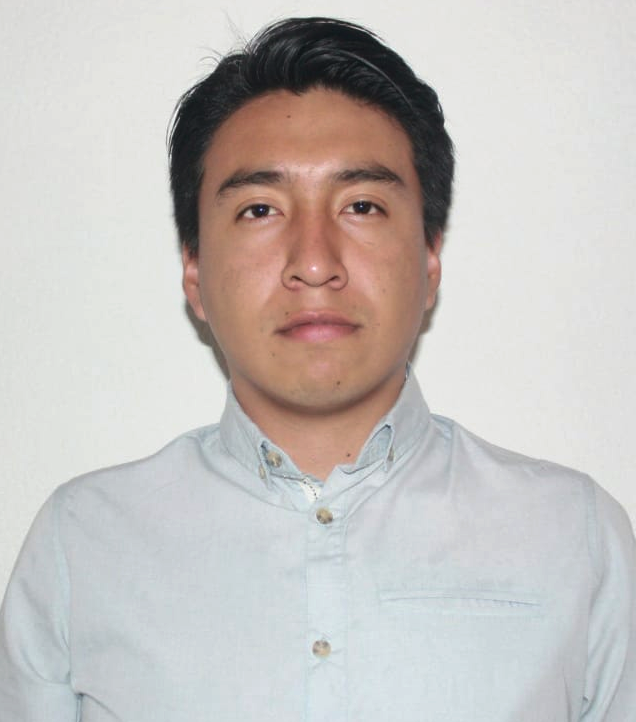
\includegraphics[width=3.9cm]{jejejejejej.png}
  \section{Tel \& LinkedIn}
    +52 55 3248 1649
    01 595 922 2525
\href{https://www.linkedin.com/in/jazzzflores/}{jazzzflores/}    
    ~
  \section{Mail}
    \href{mailto:jazzesfm@gmail.com}{\textbf{jazzesfm@}\\gmail.com}
    \href{mailto:jfloresr1302@alumno.ipn.mx}{\textbf{jfloresr1302@}\\alumno.ipn.mx}

    ~
  \section{Web \& Git}
    \href{https://medium.com/@jazzesfm}{JazzzFlorent.com}
   \href{https://www.hackthebox.eu/profile/171317}{hackthebox/CodexReck}
   \href{https://platzi.com/@jazzfm/}{platzi/@jazzfm}   
   \href{https://github.com/JazzzFM}{github.com/JazzzFM}
   \href{https://gitlab.com/u/JazzzFM?}{gitlab.com/JazzzFM}
    ~
 % use  \hspace{} or \vspace{} to change bubble size, if needed
  \section{Programming}
    \smartdiagram[bubble diagram]{
        \textbf{C \& C+},
        \textbf{Java},
        \textbf{Octave},
        \textbf{PLC},
        \textbf{HTML},
        \textbf{Bash}
    }
    ~
  \section{Cualidades Personales}
    \smartdiagram[bubble diagram]{
        \textbf{Auto-}\\\textbf{didacta},
        \textbf{Empatía},
        \textbf{Analisis},
        \textbf{Renovación},
        \textbf{Proactividad},
        \textbf{Rigor},
        \textbf{Orden}
    }
    ~
\end{aside}
~

\section{Educación.}
\begin{entrylist}
  \entry
    {2013- 2016.}
    {Tećnico en Sistemas de Control Eléctrico.}
    {\href{https://cecyt3.ipn.mx}{<< CECyT 3 - IPN >>}}
{ Fue en esta parte de mi vida donde adquirí conocimientos introductorios, fuertes y rigurosos, tanto cientificos como técnicos. Aquí se hicieron crecer mis habilidades para diseñar, contruir y manejar protocolos de control para la construcción de prototipos de ende tecnológico con el manejo de distintas herramientas importantes propias del área como lo fueron; SolidWorks, Autocad, HTML básico, estación de soldar y sierras eléctricas. Un acontecimiento importante fue mi primer acercamiento a la programación, en el lenguaje C para microcontroladores y lenguaje escalera para PLC.
    \\}
  \entry
    {2016 - 2020}
    {Licenciatura en Física y Matemáticas.}
    {\href{https://www.esfm.ipn.mx}{<< ESFM - IPN >>}}
    {
    Creo fervientemente que no puder haber elegido una mejor carrera para mí, ha sido reconfortante encontrar esas bases sólidas en matemáticas, que me han ayudado principalmente en la programación, y ese amor por el entendimeinto en general de hechos en la naturaleza. El rigor ha sido la guía principal. Lo que me ha permitido compartir, como profesor, mis conocimientos. He visto la importancia de las comunidades, ya que me han abierto las puertas a diversas oportunidades. Fue aqui donde le agarré el gusto al sistema operativo GNU/Linux, al \textit{Free Software} como al \textit{Open Source}, así como a la seguridad informática.  
    \\}
  
\end{entrylist}

\section{Experiencia.}
\begin{entrylist}
    
    \entry
    {2016}
    {Tésis y Trabajo Terminal: }
    {\href{https://cecyt3.ipn.mx}{<< CECyT 3 - IPN >>}}
    { \textbf{Desarrollo de un Módulo Móvil-Automático de Limpieza.}
    \href{https://www.youtube.com/watch?v=zbDAjEfyKrY}{   \textit{<< Ver Vídeo >>}}
    \\
    \textbf{Supervisores}: M.C. Libia Zoraida Torres e Ing. Juan Ignacio Lima Velazco.\\
    \textbf{Descripción}: Un módulo móvil que, en conjunto con un brazo robótico, conforme un solo robot de limpieza que facilite la realización de tareas domésticas, en específico barrer y trapear, mediante la implementación de mecanismos y sistemas automatizados. \href{https://drive.google.com/file/d/12gbIxFkS-cf5gG1gvyKvA9u7UeBOZkpy/view?usp=sharing}{\textit{<< Ver Tésis >>}}\\
    }
  \entry
    {2015 - 2016}
    {Servicio Social:}
    {\href{https://cecyt3.ipn.mx}{<< CECyT 3 - IPN >>}}
    {\textbf{Programa de Apoyo al Docente del Área de Investigación.}
    \\
    Desarrollé con SolidWorks engranes, tornillos y piezas diversas para un proyecto que contemplaba un brazo robótico, coticé el costos para el proyeto de un dron, con ayuda de alumnos investigadores diseñamos el control electrónico de motores y la interfaz para controlar un robot a distancia.\\}
    \entry
    {2018 - 2019}
    {Docente de Medio Tiempo }
    {\href{https://www.facebook.com/Kaleido.edu/}{<< Kaleido Regualrizaciones >>}}
    { Desempeñé el cargo como profesor para alumnos de edades diversas, impartiendo asignaturas de mi área, matemáticas y física, en todos los niveles,  pero también otras que no lo eran, como inglés, español, geografía, historia universal y de méxico, finanzas, etc. Asímsmo impartí un curso de preparación para ingresar a la \textbf{UNAM}. \href{https://drive.google.com/file/d/1w9CVCy-d3eIhm1HHeQm1GP25B_DY_1Zo/view?usp=sharing}{\textit{<< Ver Constancia Laboral >>}} \\}
    
\end{entrylist}
\newpage

\begin{aside}
~
~
~
 

  \section{OS Preferidos}
    \textbf{GNU/Linux}
\includegraphics[scale=0.40]{img/5stars.png}
    \textbf{Windows}
\includegraphics[scale=0.40]{img/3stars.png}
    \textbf{MacOS}
\includegraphics[scale=0.40]{img/2stars.png}
    ~
  \section{Idiomas}
    \textbf{Español}
\includegraphics[scale=0.40]{img/5stars.png}
    \textbf{Inglés}
\includegraphics[scale=0.40]{img/3stars.png}
    \textbf{Francés}
\includegraphics[scale=0.40]{img/2stars.png}
    \textbf{Japonés}
\includegraphics[scale=0.40]{img/1stars.png}
    \textbf{Aleman}
\includegraphics[scale=0.40]{img/1stars.png}
    
    ~
    ~
    ~
    ~
    ~
    ~
    ~
    ~
    ~
    \begin{figure}
        \centering
     
\includegraphics[width=.55\textwidth,center]{CAESCOM.jpg}
\label{fig:my_label}
    \end{figure}
    ~
    ~
    \begin{figure}
        \centering
     
\includegraphics[width=.52\textwidth,center]{cin.jpeg}
     \end{figure}
    ~
    ~
    \begin{figure}
        \centering
     
\includegraphics[width=.55\textwidth,center]{CSIESCOM.png}
\label{fig:my_label}
    \end{figure}
    ~
    ~ 

     \begin{figure}
        \centering
     
\includegraphics[width=.75\textwidth,center]{ibm.png}
    \end{figure}
    ~
\end{aside}
\\

\section{Objetivo Profesional.}
Busco desempeñarme plenamente como programador o pentester jr. esto en un área de trabajo diversa, muy abierta, donde pueda crecer y aprender continuamente así como compartir mi conocimiento hacia un equipo y ofrecer mis habilidades lógico-matemáticas siempre con rigor y orden.

\section{Manejo de Software.}
• Uso básico de los Sistemas Operativos GNU/Linux y Windows.\\
• Uso Intermedio de Terminal con Bash.\\
• Uso básico de VIM y Emacs.\\
• Uso básico de paquetería Officce y LibreOffice: Excel, Word, PowerPoint.\\
• Uso básico de LaTex y Octave.\\
• Uso básico de AutoCad, SolidWorks.\\
• Programación estructurada en C/C++ .\\
• Programación básica de Microcontroladores, Arduino y PLC.\\



\section{Cursos Extra-Académicos.}
\begin{entrylist}
 
  \entry{ 2019 - 1 }{Club de Algoritmia de ESCOM}{\href{https://www.cec.escom.ipn.mx/index.php/es/}{<< ESCOM - IPN >>}}{Fui miembro de Febrero a Mayo de este año, donde estudiamos temas más profundos como \textit{Dynamic programming} y \textit{Backtracking}}
  
  \entry{ 07/2019 }{Escuela de Verano de Matemáticas}
  {\href{https://www.math.cinvestav.mx}{<< CINVESTAV - IPN >>}}
  {
  Durante vacaciones de verano decidí asistir pues me interesaron temas de fontera en matemáticas y fue una gran oportunidad para conocer el trabajo de los demás y esa gran institución. Particularmente me interesé por la \textit{Criptografía} y el \textit{Súper Cómputo}, pero también la \textit{Topología} y el \textit{Álgebra}.\\
   << \href{https://drive.google.com/file/d/0BxsBj4oBVw3fMlVjQXlfOGl3VHhYUm15RlRlQXVHMHE1Nm9Z/view?usp=sharing}{\textit{Ver Constancia}} >>
  }
  
  \entry{2019 - 2}{Club de Seguridad Informática de ESCOM}{\href{https://www.cec.escom.ipn.mx/index.php/es/}{<< ESCOM - IPN >>}}
  {
  Miembro activo de tres tipos de actividades; \textit{Introducción a la Seguridad Informática}, \textit{Pentesting} y \textit{Capture the Flag}, fue aqui donde se me han abierto oportunidades de colaboración con otros estudiantes en un meetup en platzi así como iniciarme a la cultura Hacker al crear una cuenta en HackTheBox para realizar pruebas de penetración y retos}
  
  \entry{13/09/2019}{Taller Watson Studio - IBM Day}{\href{https://www.cec.escom.ipn.mx/index.php/es/}{<< ESCOM - IPN>>}}
  {
  Realicé un taller introductorio a la Inteligencia Artificial Watson donde hicimos configuraciones de algoritmos  para; categorizar un conjunto de datos, reconocimiento de imágenes y creación de un chatbot muy básico, así como entender los principios de su funcionamiento  \href{https://drive.google.com/file/d/1HZNd6Rm6PFyitDFkMpKJaU-E61z-BiQa/view?usp=sharing}{ << Ver Aquí >>}
  }
  
  
\end{entrylist}

\section{Datos de Interés.}
Me gusta escribir y leer, en genereal, crear. Me interesa la matemática como actividad creativa, como si fuera literatura, pienso en hacer un posgrado en \textit{Teoría de Números}, \textit{Criptografía}, \textit{Súper Cómputo} o \textit{Topología} en el CINVESTAV o bien en extrangero, sin embargo en este momento me interesa conocer la industria y desarrollame en ella antes, es por ello que me di a la tarea de empezar cursos en \textbf{platzi} sobre Ciber Serguridad, desarrollo con IBM - Cloud, así como desarrollo web, aprender diferentes lenguajes de programación y desarrollo personal, etc. espero pronto terminarlos.

\end{document}
